\section{Introduction}
The design of LARRE was inspired by the modular design presented by Bartenbach \textit{et. al.} \cite{7523699}.  Aliman \textit{et. al} also comprised a survey of all the existing lower limb exoskeletons currently in development; the survey gave further insight into the choice of actuators and sensors \cite{aliman2017design}. The Bartenbach design outlined the basic structure for the rehabilitation exoskeleton and improved by integrating additional sensors from the Aliman survey into the system. Additionally, the ankle-foot orthosis was moved to an overshoe joint to allow the system to don and doff with greater ease.
LARRE was designed to be a modular testing platform. Here we define modular as the ability to adjust to a person and allow for the swapping out of the joint mechanisms. LARRE's design fits the following requirements. 


\begin{enumerate}[noitemsep]
\item \textbf{Data Driven}: The kinematics and dynamics of the joints are defined by the biomechanical data. The joints must have the power to compensate for the mass of the person and the exoskeleton. 
\item \textbf{Adjustable}: The exoskeleton must be adjustable to fit the different people in order for the exoskeleton's joints to align properly to avoid putting unnatural force on a person's joints. 
\item \textbf{Modular}: The exoskeleton requires removable joints to allow for different joints testing and experimentation; therefore, universal connectors are needed to allow the swapping out of the joints. 
\item \textbf{Easy to build}: The exoskeleton needs to be easy to manufacture and assemble. The exoskeleton should be constructed from off-the-shelf material to allow researchers to build their testing and development systems. 
\item \textbf{Easy of Use}: The exoskeleton needs to be easy to use for both the clinician and the person wearing the exoskeleton. 
\end{enumerate}

 \autoref{fig:Render} shows an annotated rendering of LARRE.  Each of the major components is discussed in detail in  \autoref{sec:hip}, \autoref{sec:knee}, and \autoref{sec:ankle}. While LARRE was designed to work as a single system, the modality allowed each joint treated as a separate component and be independently designed and tested. 

\begin{figure}[h!]
    \centering
    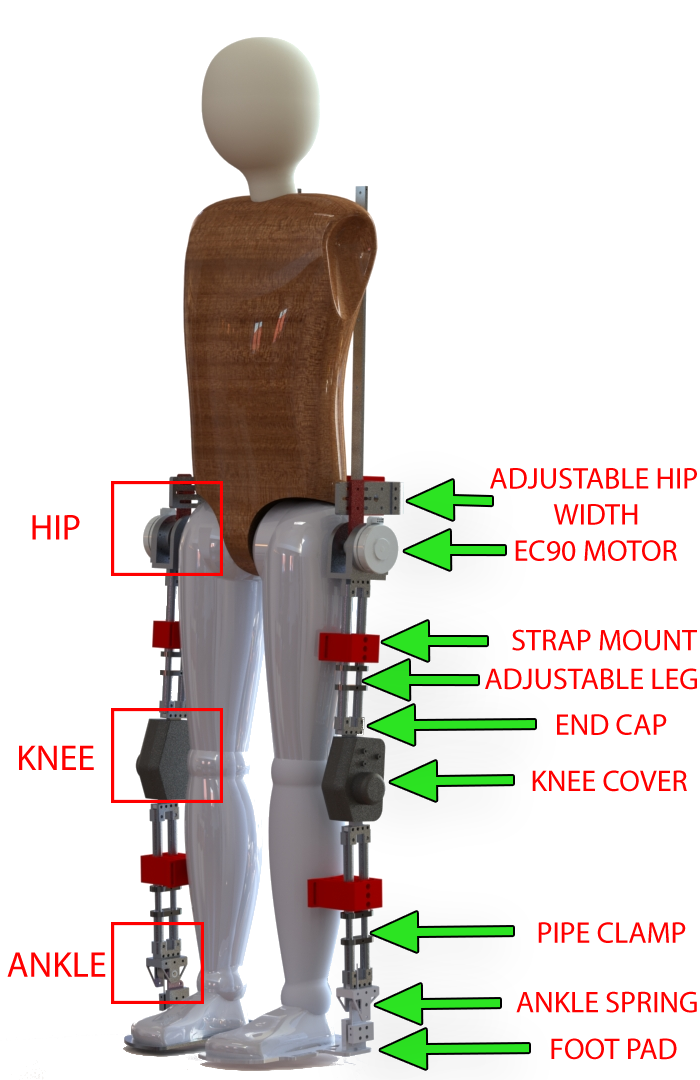
\includegraphics[scale=0.25]{images/mech_design/rendering2.png}
    \caption{Rendering of exoskeleton.}
    \label{fig:Render}
\end{figure}

